\documentclass[xcolor=x11names,compress]{beamer}
\usepackage[ngerman]{babel}
\usepackage{pgfplotstable}
\usepackage{tabularx}
\usepackage{tikz}
\usepackage{graphicx}
\usepackage{times}
\usepackage{theorem}
\usepackage{algorithm2e}
\usepackage{natbib}
\usepackage{bibentry}

\makeatletter
\let\beamer@writeslidentry@miniframeson=\beamer@writeslidentry
\def\beamer@writeslidentry@miniframesoff{%
  \expandafter\beamer@ifempty\expandafter{\beamer@framestartpage}{}% does not happen normally
  {%else
    % removed \addtocontents commands
    \clearpage\beamer@notesactions%
  }
}
\newcommand*{\miniframeson}{\let\beamer@writeslidentry=\beamer@writeslidentry@miniframeson}
\newcommand*{\miniframesoff}{\let\beamer@writeslidentry=\beamer@writeslidentry@miniframesoff}
\makeatother

\nobibliography*
\usetheme{Antibes}
\setbeamertemplate{navigation symbols}{}
\usefonttheme{serif}

% BEAMER THEME
\useoutertheme[subsection=false,shadow]{miniframes}
\useinnertheme{default}
\usepackage{palatino}

\setbeamerfont{title like}{shape=\scshape}
\setbeamerfont{frametitle}{shape=\scshape}

\setbeamercolor*{lower separation line head}{bg=white} 
\setbeamercolor*{normal text}{fg=black,bg=white} 
\setbeamercolor*{alerted text}{fg=red} 
\setbeamercolor*{example text}{fg=black} 
\setbeamercolor*{structure}{fg=black} 
 
\setbeamercolor*{palette tertiary}{fg=black,bg=white} 
\setbeamercolor*{palette quaternary}{fg=black,bg=black!10} 
% END BEAMER THEME

\pgfplotstableread{img/gausssteps/default_0.dat}\matrixdefaulta
\pgfplotstableread{img/gausssteps/default_1.dat}\matrixdefaultb
\pgfplotstableread{img/gausssteps/default_2.dat}\matrixdefaultc
\pgfplotstableread{img/gausssteps/default_3.dat}\matrixdefaultd
\pgfplotstableread{img/gausssteps/default_4.dat}\matrixdefaulte
\pgfplotstableread{img/gausssteps/default_5.dat}\matrixdefaultf
\pgfplotstableread{img/gausssteps/default_6.dat}\matrixdefaultg
\pgfplotstableread{img/gausssteps/default_7.dat}\matrixdefaulth

\pgfplotstableread{img/gausssteps/optimized_0.dat}\matrixpeoa
\pgfplotstableread{img/gausssteps/optimized_1.dat}\matrixpeob
\pgfplotstableread{img/gausssteps/optimized_2.dat}\matrixpeoc
\pgfplotstableread{img/gausssteps/optimized_3.dat}\matrixpeod
\pgfplotstableread{img/gausssteps/optimized_4.dat}\matrixpeoe
\pgfplotstableread{img/gausssteps/optimized_5.dat}\matrixpeof
\pgfplotstableread{img/gausssteps/optimized_6.dat}\matrixpeog
\pgfplotstableread{img/gausssteps/optimized_7.dat}\matrixpeoh

\definecolor{light-gray}{gray}{0.90}

\newcommand{\spymatrix}[1]{\resizebox{\columnwidth / 4}{!}{
		\begin{tikzpicture}
			\foreach \i in {0,...,7}{
					\foreach \j in {0,...,7}{
							\pgfplotstablegetelem{\i}{\j}\of#1
							\ifnum\pgfplotsretval=0
								\node[circle, minimum size=.5pt, inner sep=0pt, fill=light-gray] at (\j pt,-\i pt) {};
							\else
								\ifnum\pgfplotsretval=1
									\node[circle, minimum size=.5pt, inner sep=0pt, fill=red] at (\j pt,-\i pt) {};
								\else
									\node[circle, minimum size=.5pt, inner sep=0pt, fill=black] at (\j pt,-\i pt) {};
								\fi
							\fi
						};
				};
		\end{tikzpicture}
	}}

\newcommand{\spymatrixpresentation}[1]{\resizebox{\columnwidth}{!}{
		\begin{tikzpicture}
			\foreach \i in {0,...,7}{
					\foreach \j in {0,...,7}{
							\pgfplotstablegetelem{\i}{\j}\of#1
							\ifnum\pgfplotsretval=0
								\node[circle, minimum size=.5pt, inner sep=0pt, fill=light-gray] at (\j pt,-\i pt) {};
							\else
								\ifnum\pgfplotsretval=1
									\node[circle, minimum size=.5pt, inner sep=0pt, fill=red] at (\j pt,-\i pt) {};
								\else
									\node[circle, minimum size=.5pt, inner sep=0pt, fill=black] at (\j pt,-\i pt) {};
								\fi
							\fi
						};
				};
		\end{tikzpicture}
	}}


\title{Platzeffiziente Erkennung von chordalen Graphen}
\subtitle{Seminar \glqq{}Algorithmen und Datenstrukturen\grqq{}}
\author{Konstantin Fickel}
\date{Sommersemester 2018}

\begin{document}

\begin{frame}
	\begin{overprint}
		\onslide<2-5>\begin{block}{Chordaler Graph}
			\( G \) ist chordal, wenn jeder Kreis mit mindestens \( 4 \) Knoten eine Sehne besitzt.
		\end{block}
	\end{overprint}
	\begin{center}
		\begin{overprint}
			\onslide<1-2>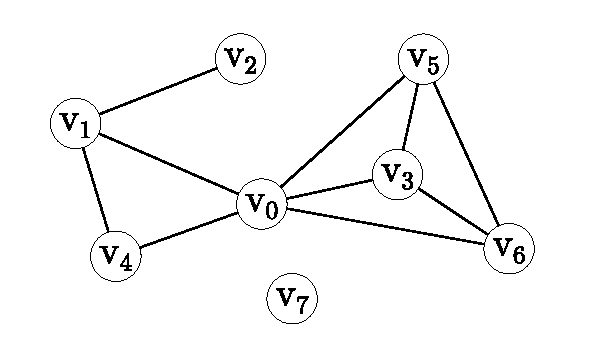
\includegraphics[scale=1.0]{img/graph/chordalsimple.pdf}
			\onslide<3>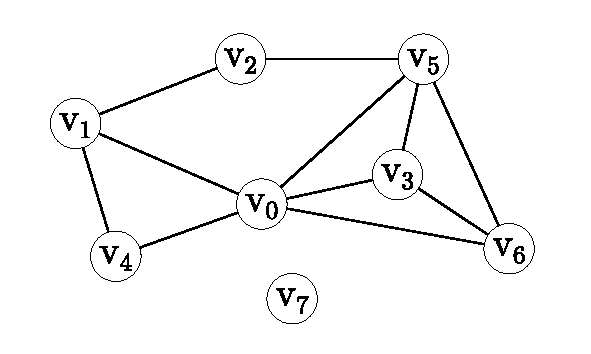
\includegraphics[scale=1.0]{img/graph/chordalnot.pdf}
			\onslide<4>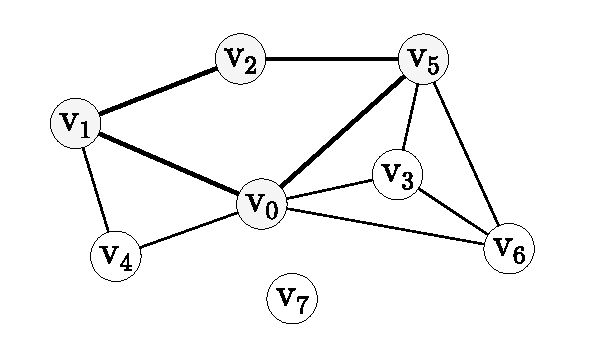
\includegraphics[scale=1.0]{img/graph/chordalnot_highlighted.pdf}
			\onslide<5>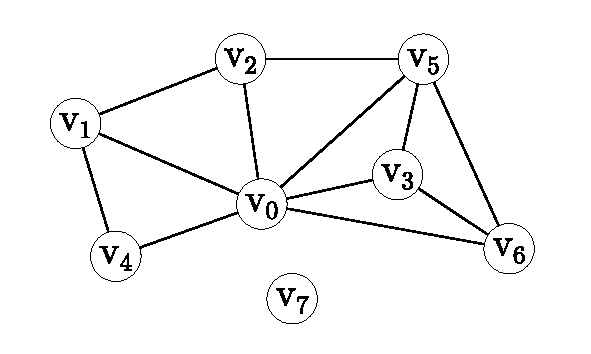
\includegraphics[scale=1.0]{img/graph/chordalsimple2.pdf}
		\end{overprint}
	\end{center}
\end{frame}

\begin{frame}
	\titlepage
\end{frame}

\bgroup
\setbeamercovered{transparent=25}
\begin{frame}
	\frametitle{Outline}
	\tableofcontents[pausesections]
\end{frame}
\egroup

\begin{frame}
	\begin{columns}
		\column{0.6\textwidth}
		\bibentry{sankardeep}
		\column{0.4\textwidth}
		\fbox{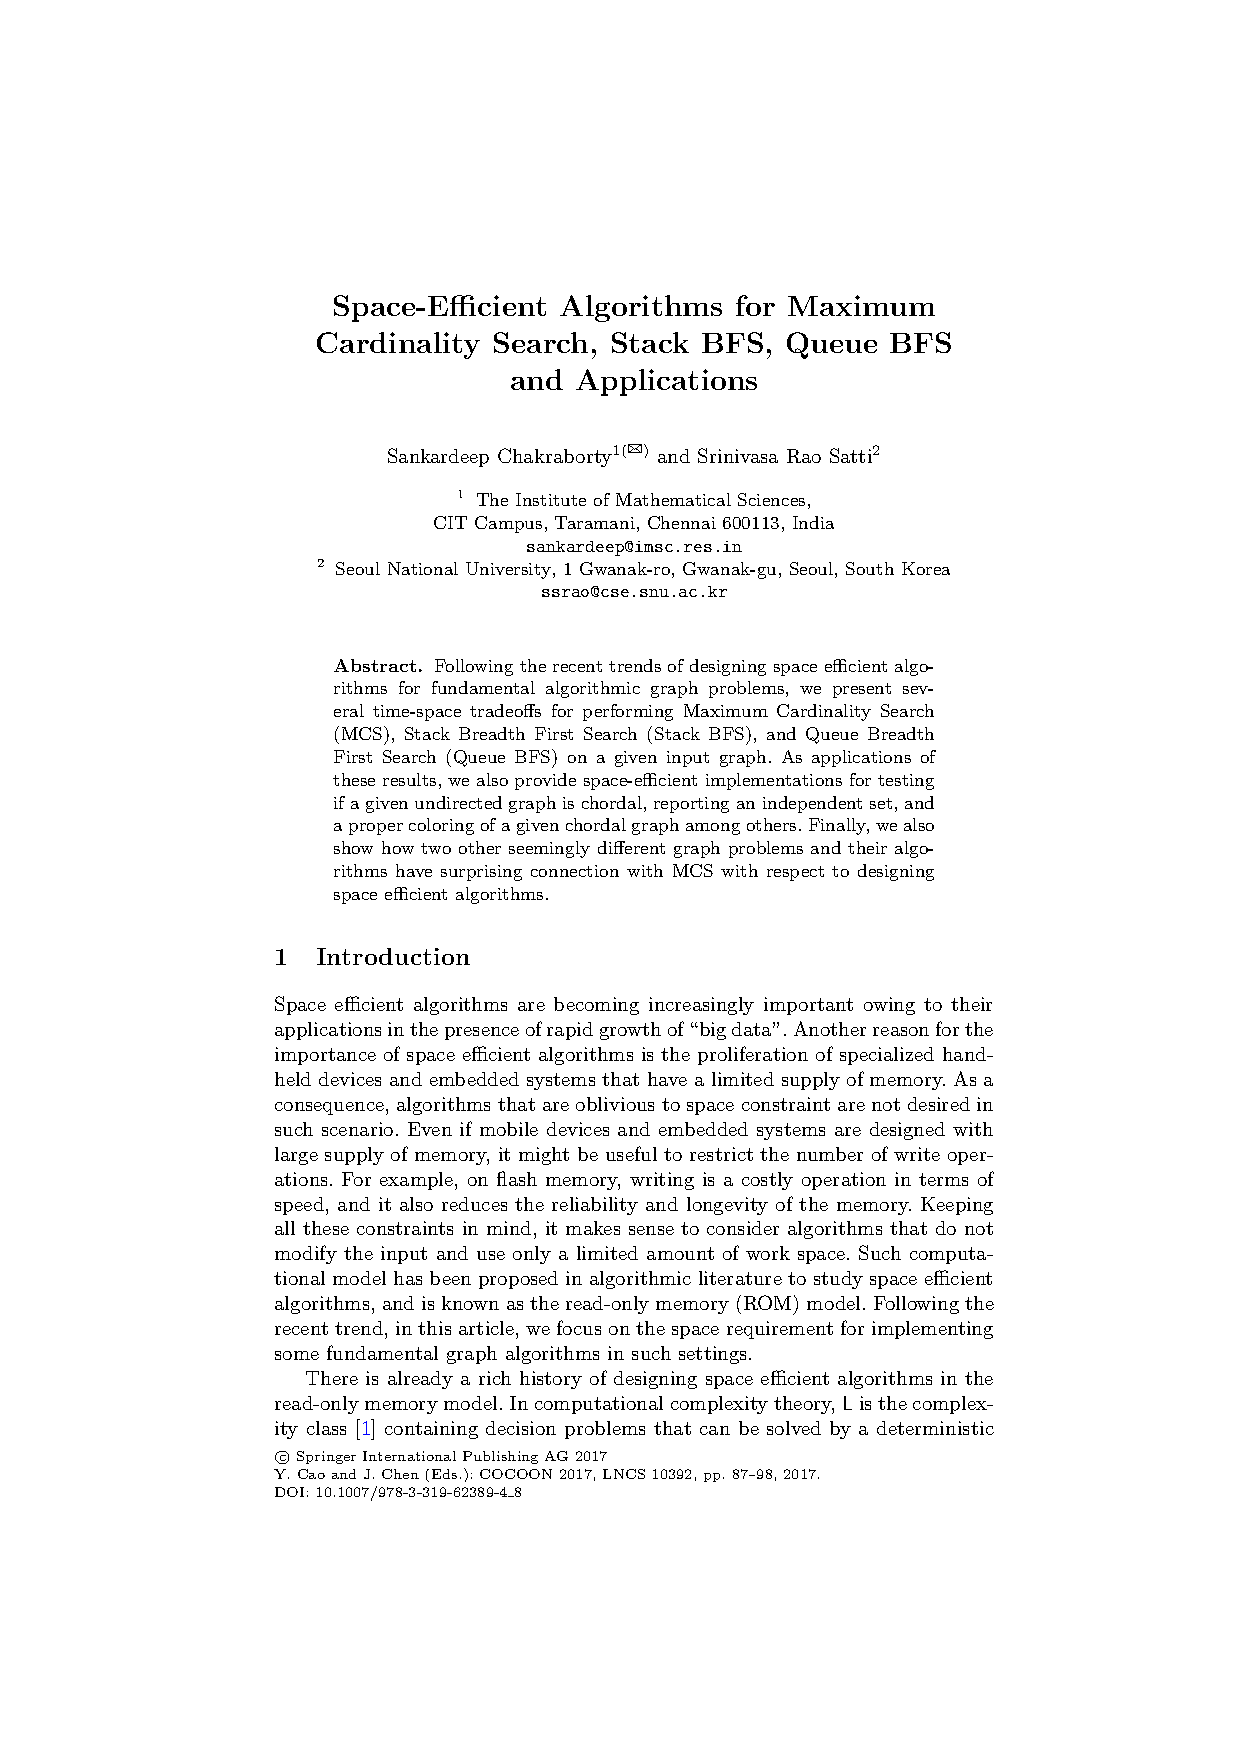
\includegraphics[width = 0.98\textwidth]{img/sources/spaceefficient.pdf}}
	\end{columns}
\end{frame}

\begin{frame}
	\begin{columns}
		\column{0.6\textwidth}
		\bibentry{golumbic}
		\column{0.4\textwidth}
		\fbox{
\includegraphics[width = 0.98\textwidth]{img/sources/golumbic.pdf}}
	\end{columns}
\end{frame}

\begin{frame}
	\begin{columns}
		\column{0.6\textwidth}
		\bibentry{tarjanyannakakis}
		\column{0.4\textwidth}
		\fbox{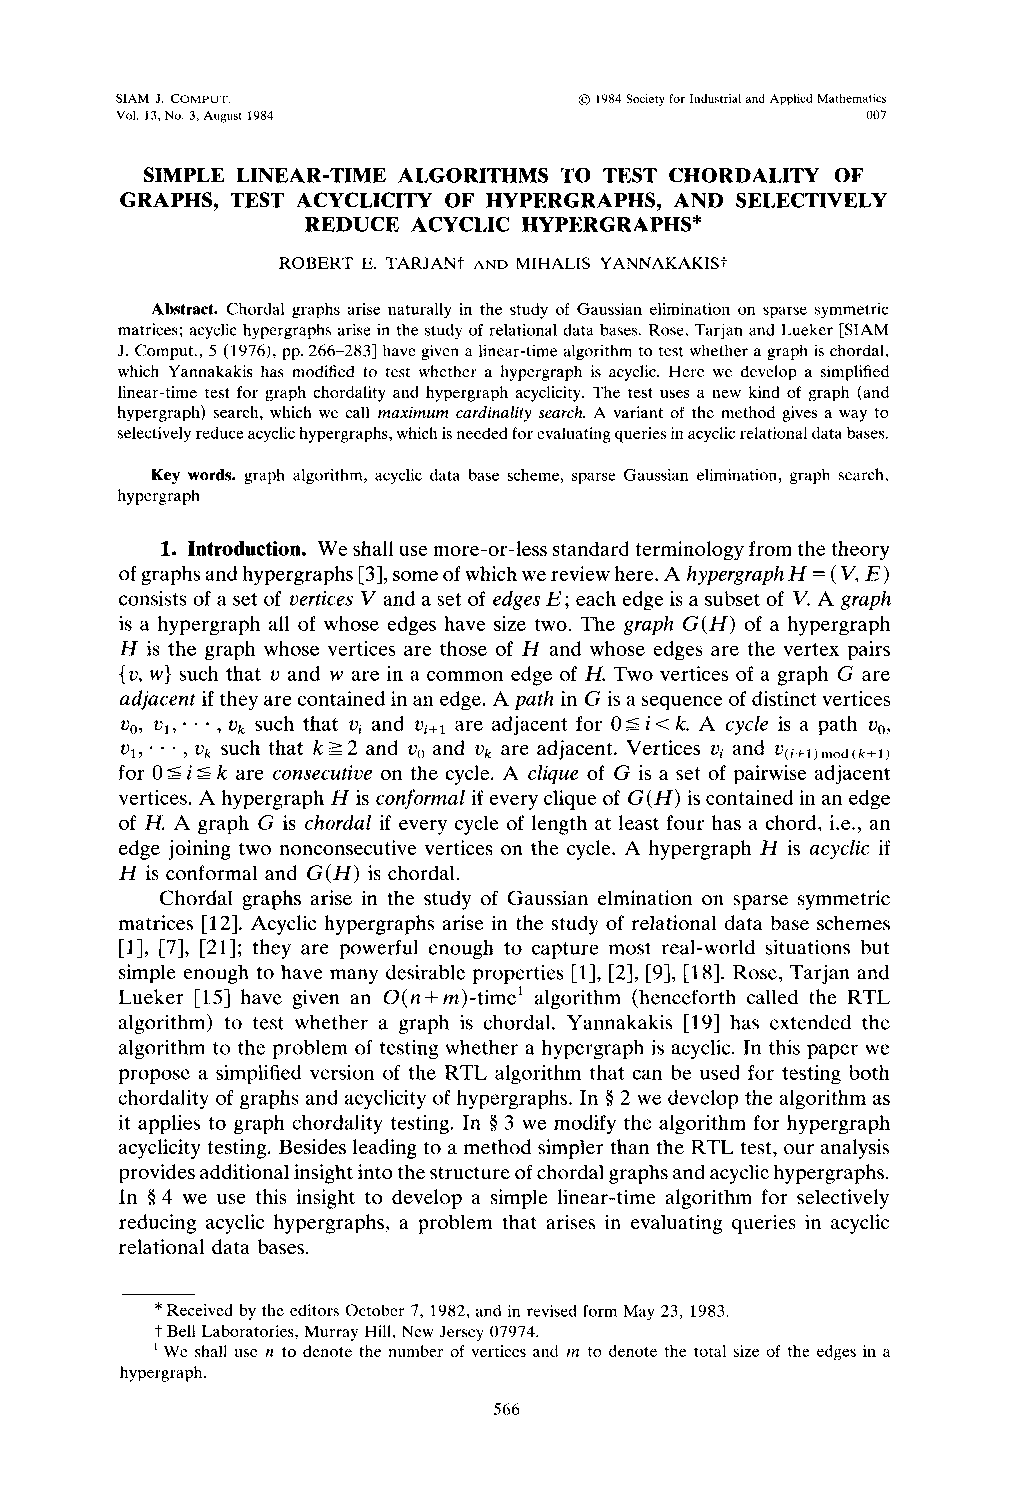
\includegraphics[width = 0.98\textwidth]{img/sources/simplelineartime.pdf}}
	\end{columns}
\end{frame}

\section{Perfekte Eliminations-Reihenfolgen}
\begin{frame}
	\begin{block}{Simplizialer Knoten}
		Ein simplizialer Knoten \( v \) in einem Graphen \( G \) ist ein Knoten, dessen Nachbarn einen vollständigen Teilgraphen \( G \left[\textnormal{Adj} \left( v \right) \right] \) induzieren.
	\end{block}
	\begin{overprint}
		\onslide<1>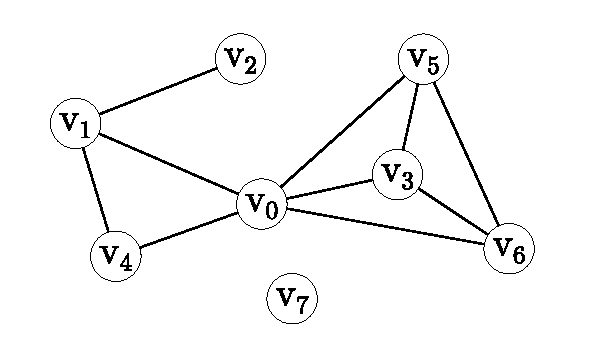
\includegraphics[scale=1.0]{img/graph/chordalsimple.pdf}
		\onslide<2>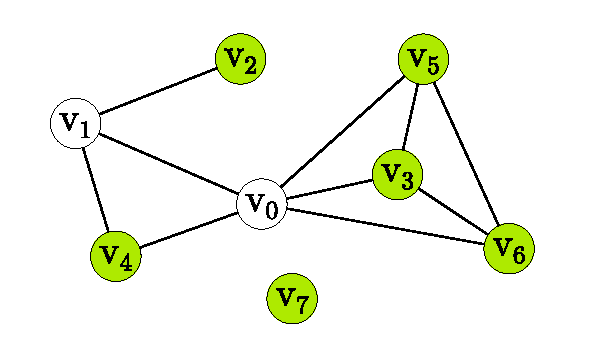
\includegraphics[scale=1.0]{img/graph/simplizial.pdf}
	\end{overprint}
\end{frame}

\begin{frame}
	\begin{block}{Perfekte Eliminations-Reihenfolge}
		Eine Reihenfolge \( \sigma \) auf \( G = \left( V, E \right) \) ist eine perfekte Eliminations-Reihenfolge, wenn für jedes \( i \in \left\lbrace 1, \ldots, \left| V \right| \right\rbrace \) der Knoten \( \sigma \left( i \right) \) simplizial im Teilgraph \( G \left[ \left\lbrace \sigma \left( i \right), \ldots, \sigma \left( \left| V \right| \right) \right\rbrace \right] \) ist.
	\end{block}
	\begin{center}
		\begin{overprint}
			\onslide<1>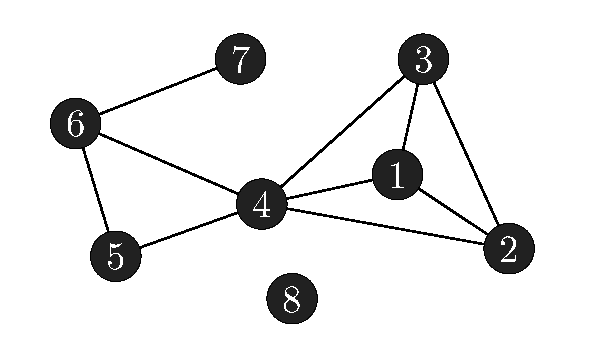
\includegraphics[scale=1.0]{img/graph/peo/01.pdf}
			\onslide<2>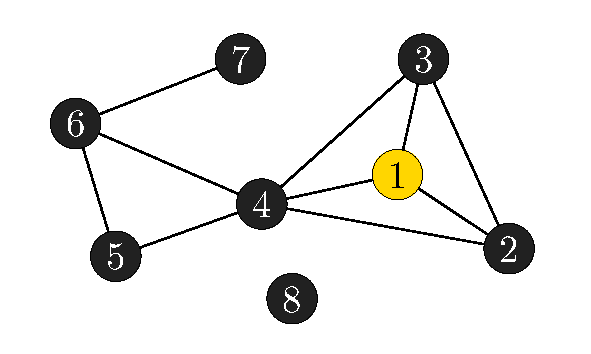
\includegraphics[scale=1.0]{img/graph/peo/02.pdf}
			\onslide<3>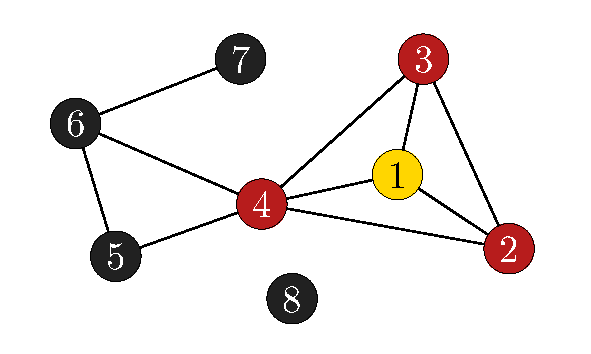
\includegraphics[scale=1.0]{img/graph/peo/03.pdf}
			\onslide<4>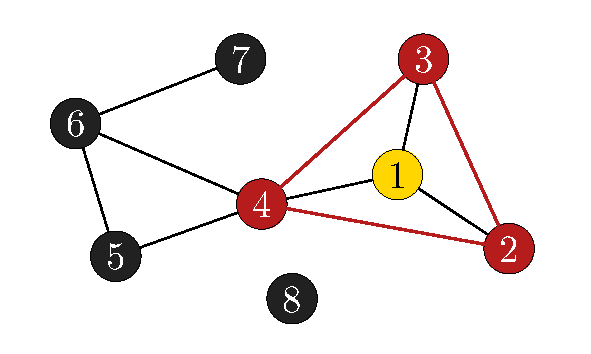
\includegraphics[scale=1.0]{img/graph/peo/04.pdf}
			\onslide<5>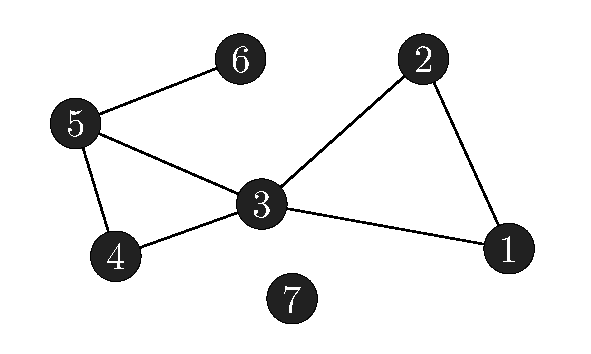
\includegraphics[scale=1.0]{img/graph/peo/05.pdf}
			\onslide<6>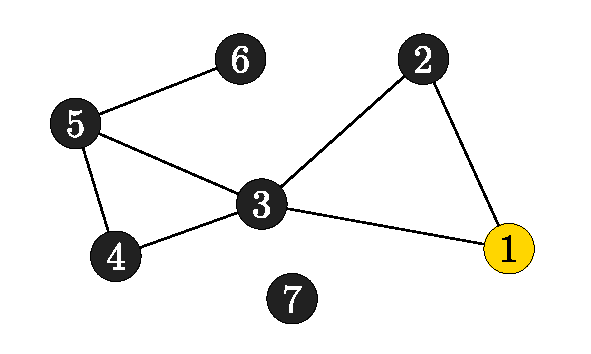
\includegraphics[scale=1.0]{img/graph/peo/06.pdf}
			\onslide<7>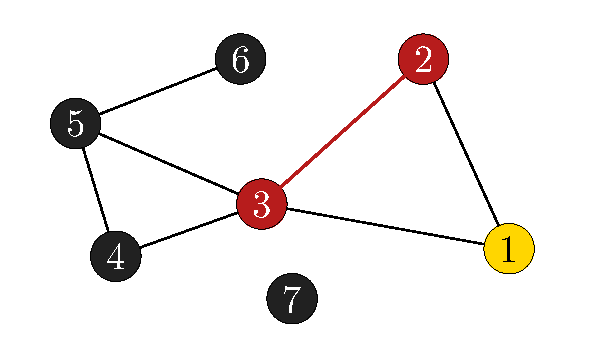
\includegraphics[scale=1.0]{img/graph/peo/07.pdf}
			\onslide<8>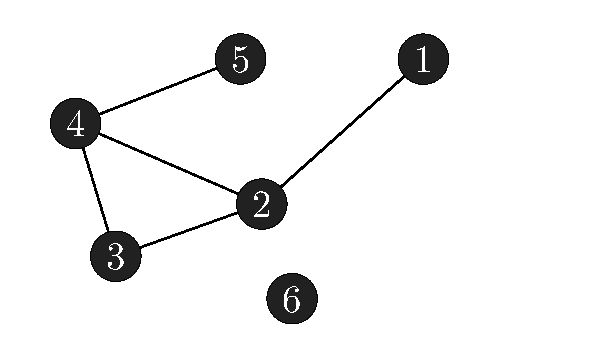
\includegraphics[scale=1.0]{img/graph/peo/08.pdf}
			\onslide<9>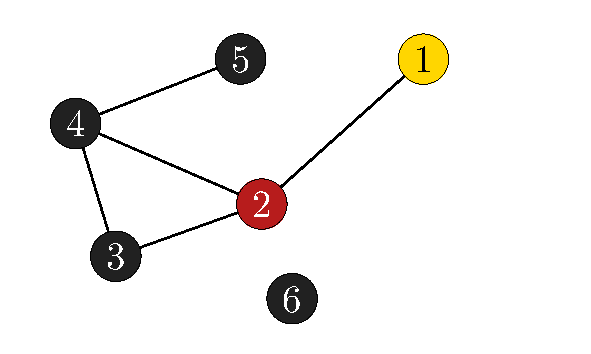
\includegraphics[scale=1.0]{img/graph/peo/09.pdf}
			\onslide<10>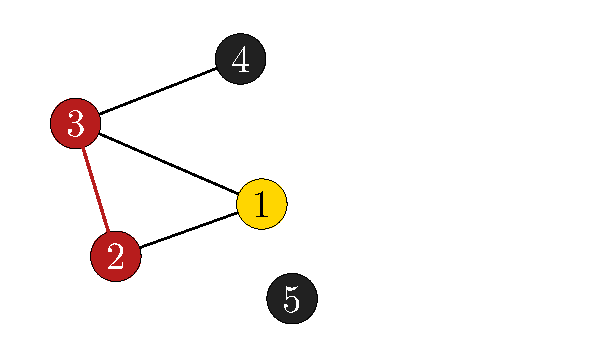
\includegraphics[scale=1.0]{img/graph/peo/10.pdf}
			\onslide<11>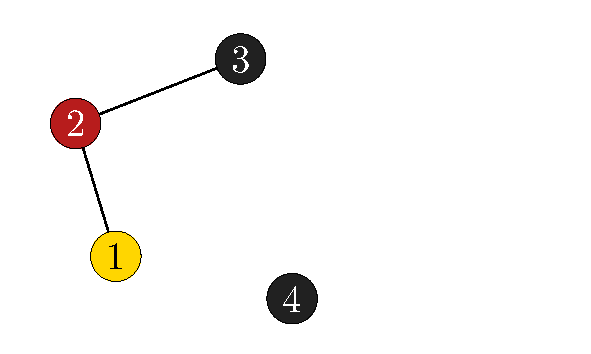
\includegraphics[scale=1.0]{img/graph/peo/11.pdf}
			\onslide<12>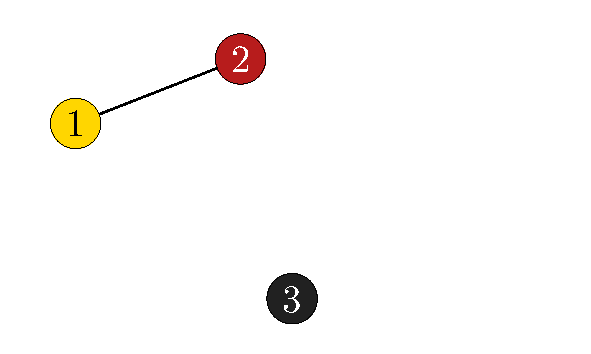
\includegraphics[scale=1.0]{img/graph/peo/12.pdf}
			\onslide<13>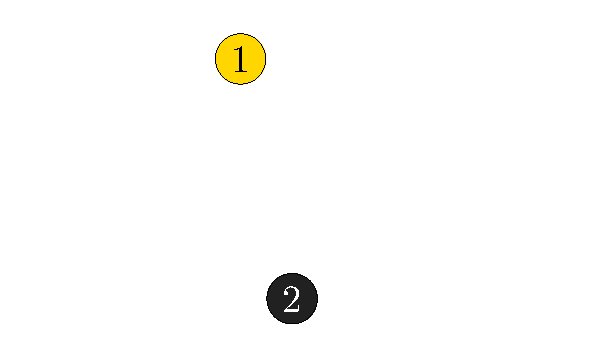
\includegraphics[scale=1.0]{img/graph/peo/13.pdf}
			\onslide<14>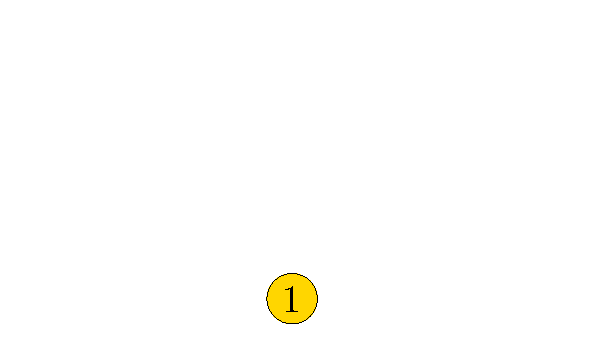
\includegraphics[scale=1.0]{img/graph/peo/14.pdf}
			\onslide<15>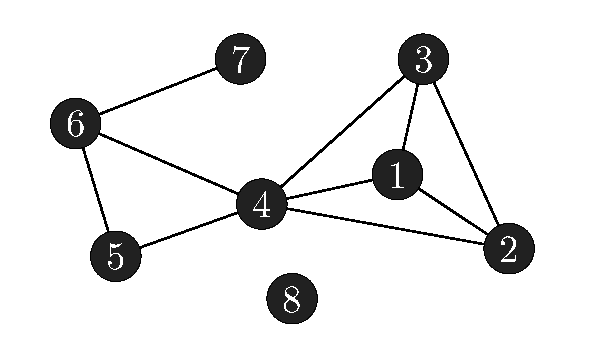
\includegraphics[scale=1.0]{img/graph/peo/01.pdf}
			% Genau genommen gibt es 6084 Möglichkeiten
			\onslide<16>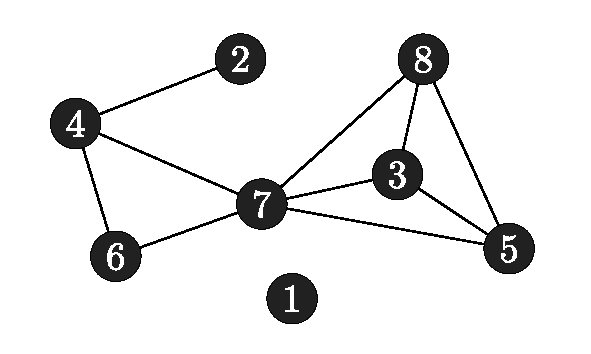
\includegraphics[scale=1.0]{img/graph/peo_alternative.pdf}
		\end{overprint}
	\end{center}
\end{frame}

\begin{frame}
	\begin{block}{Knotentrenner}
		Ein Knotentrenner \( S \) der Knoten \( a, b \in V \) ist eine Teilmenge \( S \subseteq V \) mit \( a, b \not\in S \), bei dem sich \( a \) und \( b \) in verschiedenen Zusammenhangskomponenten von \( G \left[ V \setminus S \right] \) befinden.
	\end{block}
	\begin{center}
		\begin{overprint}
			\onslide<1>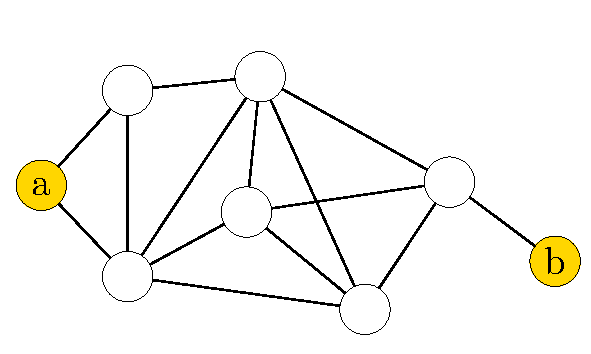
\includegraphics[scale=1.0]{img/graph/nodeseparator/01.pdf}
			\onslide<2>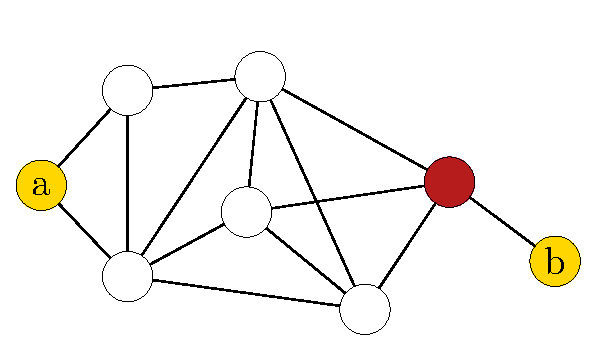
\includegraphics[scale=1.0]{img/graph/nodeseparator/02.pdf}
			\onslide<3>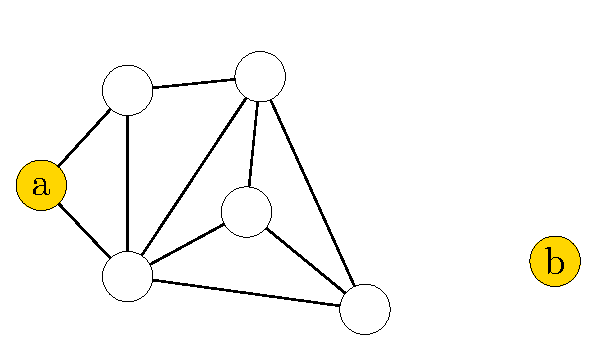
\includegraphics[scale=1.0]{img/graph/nodeseparator/03.pdf}
			\onslide<4>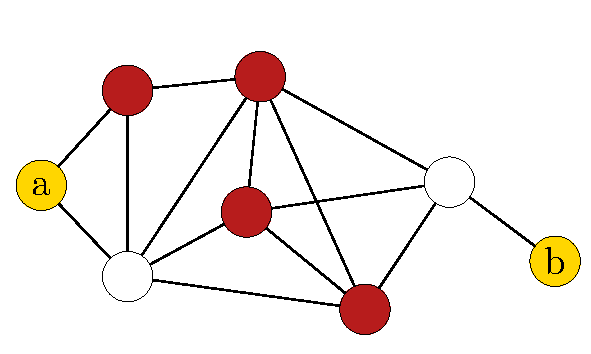
\includegraphics[scale=1.0]{img/graph/nodeseparator/04.pdf}
		\end{overprint}
	\end{center}
\end{frame}

\begin{frame}
	\begin{block}{Minimaler Knotentrenner}
		\( S \) ist ein minimaler Knotentrenner, falls diese Aussage für kein \( T \subsetneq S \) gilt.
	\end{block}
	\begin{center}
		\begin{overprint}
			\onslide<1>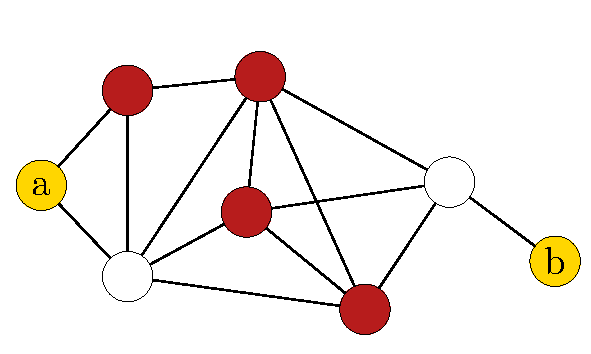
\includegraphics[scale=1.0]{img/graph/nodeseparator/04.pdf}
			\onslide<2>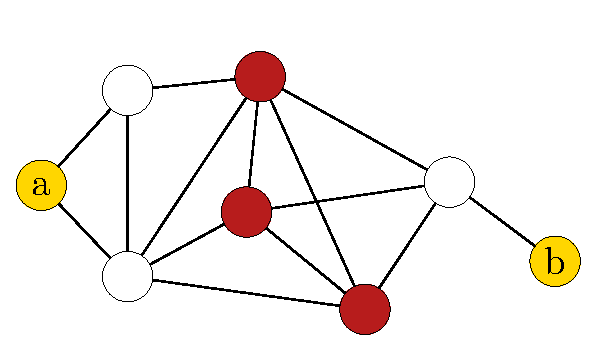
\includegraphics[scale=1.0]{img/graph/nodeseparator/05.pdf}
		\end{overprint}
	\end{center}
\end{frame}

\begin{frame}
	\begin{block}{Lemma 1}
		Sei \( G = \left( V, E \right) \) ein chordaler Graph. Dann ist der induzierte Teilgraph \( G \left[ S \right] \) zu jedem minimalen Knotentrenner \( S \subseteq V \) vollständig.
	\end{block}
	\begin{center}
		\begin{overprint}
			\onslide<2>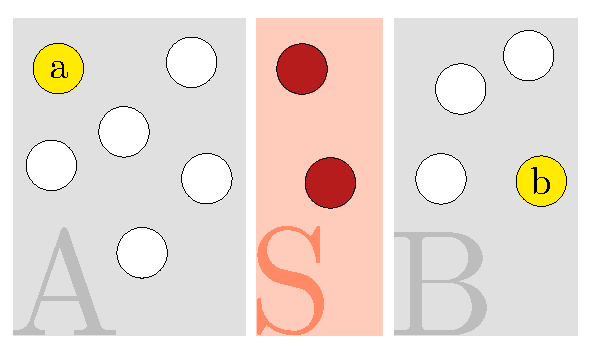
\includegraphics[scale=1.0]{img/graph/nodeseparator/proof/01.pdf}
			\onslide<3>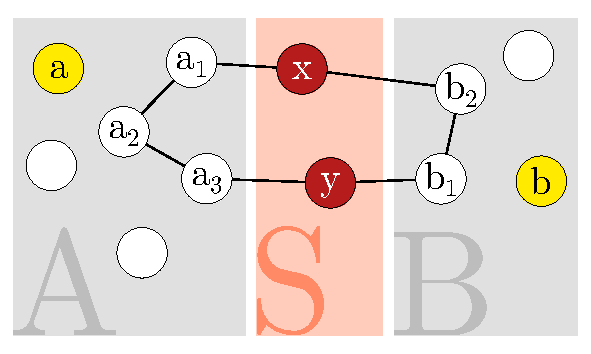
\includegraphics[scale=1.0]{img/graph/nodeseparator/proof/02.pdf}
			\onslide<4>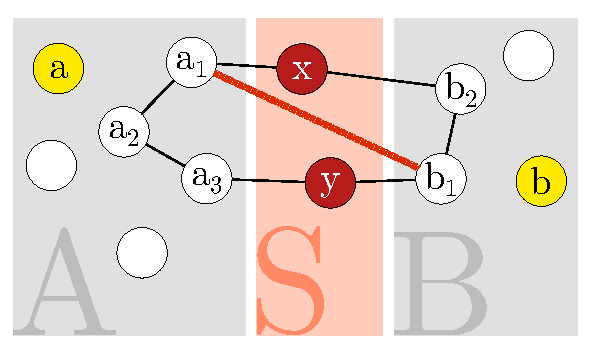
\includegraphics[scale=1.0]{img/graph/nodeseparator/proof/03.pdf}
			\onslide<5>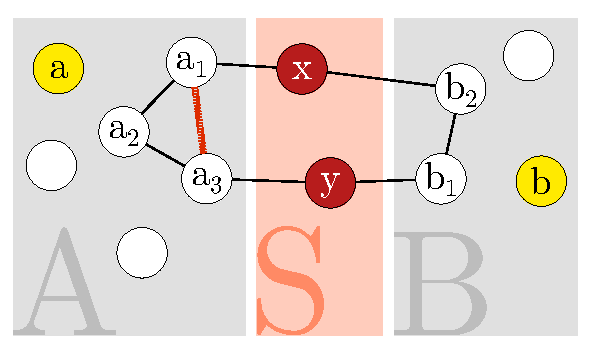
\includegraphics[scale=1.0]{img/graph/nodeseparator/proof/04.pdf}
			\onslide<6>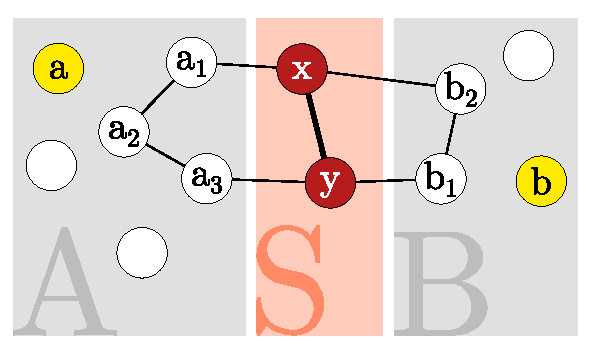
\includegraphics[scale=1.0]{img/graph/nodeseparator/proof/05.pdf}
			\onslide<7>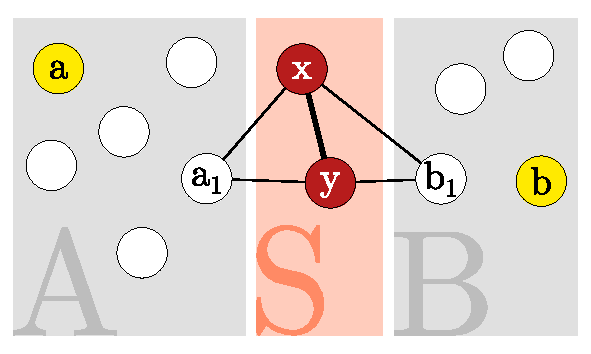
\includegraphics[scale=1.0]{img/graph/nodeseparator/proof/06.pdf}
		\end{overprint}
	\end{center}
\end{frame}

\begin{frame}
	\begin{block}{Lemma 2}
		Jeder chordale Graph \( G = \left( V, E \right) \) besitzt einen simplizialen Knoten. Falls \( G \) nicht vollständig ist, dann besitzt dieser zwei nicht-benachbarte simpliziale Knoten.
	\end{block}
	\begin{itemize}
		\item<2->[IV] Für jeden chordalen Graphen \( G = \left( V, E \right) \) mit \( \left| V \right| \leq t \) gelte, dass \( G \) entweder vollständig ist oder zwei nicht-benachbarte simpliziale Knoten besitzt.
	\end{itemize}
	\begin{overprint}
		\onslide<3>
		\( t = 1 \)

		
\includegraphics[scale=1.0]{img/graph/simplicialproof/ia.pdf}
		\onslide<4>
		\( t \Rightarrow t + 1 \)

		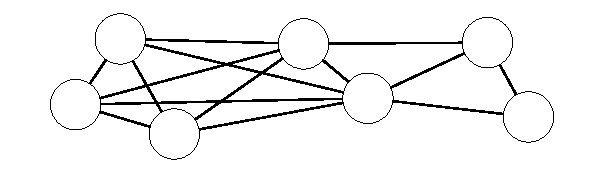
\includegraphics[scale=1.0]{img/graph/simplicialproof/iv-01.pdf}
		\onslide<5>
		\( t \Rightarrow t + 1 \)

		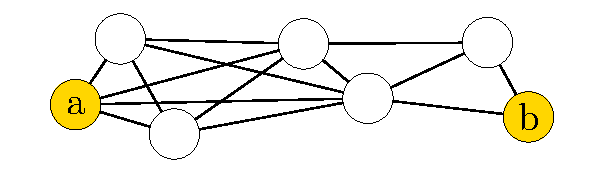
\includegraphics[scale=1.0]{img/graph/simplicialproof/iv-02.pdf}
		\onslide<6>
		\( t \Rightarrow t + 1 \)

		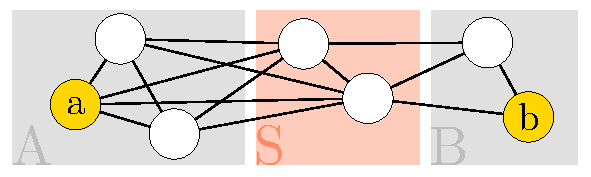
\includegraphics[scale=1.0]{img/graph/simplicialproof/iv-03.pdf}
		\onslide<7>
		\( t \Rightarrow t + 1 \)

		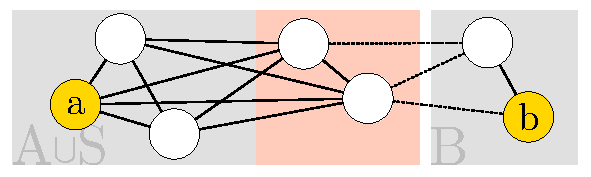
\includegraphics[scale=1.0]{img/graph/simplicialproof/iv-04.pdf}
		\onslide<8>
		\( t \Rightarrow t + 1 \)

		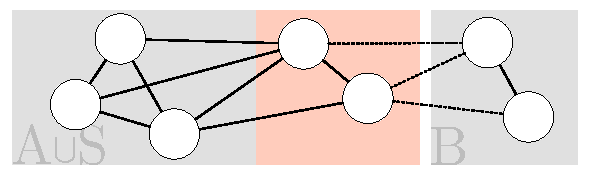
\includegraphics[scale=1.0]{img/graph/simplicialproof/iv-05.pdf}
		\onslide<9>
		\( t \Rightarrow t + 1 \)

		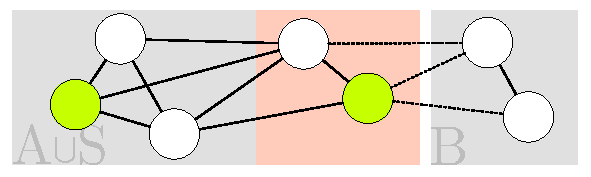
\includegraphics[scale=1.0]{img/graph/simplicialproof/iv-06.pdf}
		\onslide<10>
		\( t \Rightarrow t + 1 \)

		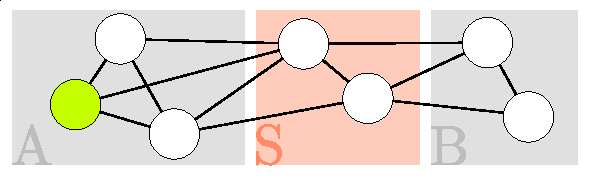
\includegraphics[scale=1.0]{img/graph/simplicialproof/iv-07.pdf}
		\onslide<11>
		\( t \Rightarrow t + 1 \)

		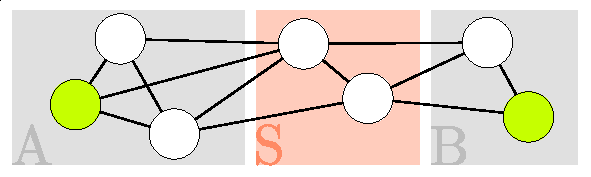
\includegraphics[scale=1.0]{img/graph/simplicialproof/iv-08.pdf}
	\end{overprint}
\end{frame}

\begin{frame}
	\begin{block}{Satz 1}
		Sei \( G \) ein ungerichteter Graph. \( G \) ist chordal genau dann, wenn für \( G \) eine perfekte Eliminations-Reihenfolge \( \sigma \) existiert.
	\end{block}
	\begin{overprint}
		\onslide<2>
		\( \Rightarrow \)

		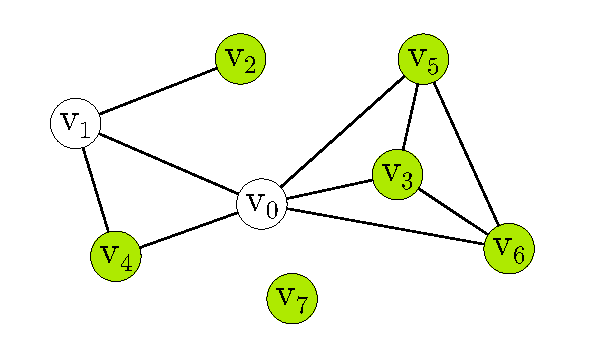
\includegraphics[scale=1.0]{img/graph/simplicialconstruction/01.pdf}
		\onslide<3>
		\( \Rightarrow \)

		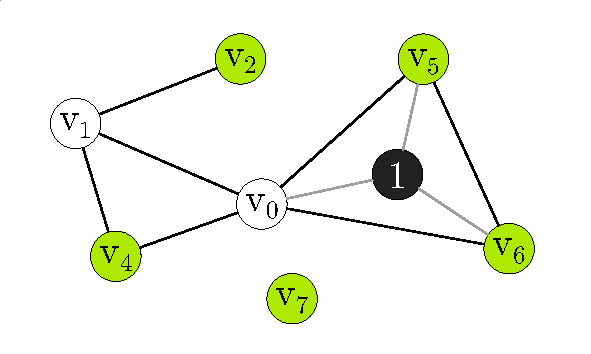
\includegraphics[scale=1.0]{img/graph/simplicialconstruction/02.pdf}
		\onslide<4>
		\( \Rightarrow \)

		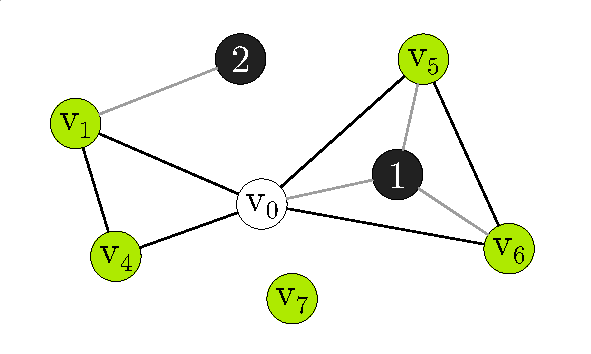
\includegraphics[scale=1.0]{img/graph/simplicialconstruction/03.pdf}
		\onslide<5>
		\( \Rightarrow \)

		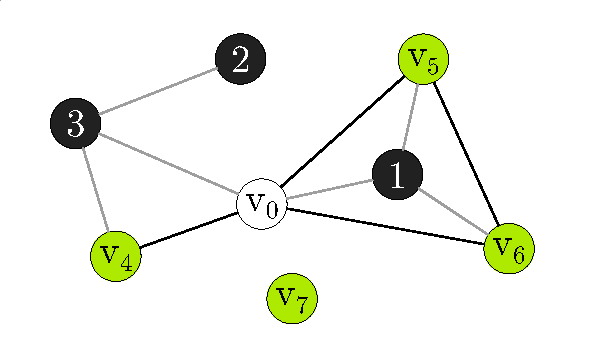
\includegraphics[scale=1.0]{img/graph/simplicialconstruction/04.pdf}
		\onslide<6>
		\( \Rightarrow \)

		\includegraphics[scale=1.0]{img/graph/simplicialconstruction/05.pdf}
		\onslide<7>
		\( \Rightarrow \)

		\includegraphics[scale=1.0]{img/graph/simplicialconstruction/06.pdf}
		\onslide<8>
		\( \Rightarrow \)

		\includegraphics[scale=1.0]{img/graph/simplicialconstruction/07.pdf}
		\onslide<9>
		\( \Rightarrow \)

		\includegraphics[scale=1.0]{img/graph/simplicialconstruction/08.pdf}
		\onslide<10>
		\( \Rightarrow \)

		\includegraphics[scale=1.0]{img/graph/simplicialconstruction/09.pdf}
		\onslide<11>
		\( \Leftarrow \)

		\includegraphics[scale=1.0]{img/graph/nodes/01.pdf}
		\onslide<12>
		\( \Leftarrow \)

		\includegraphics[scale=1.0]{img/graph/nodes/02.pdf}
		\onslide<13>
		\( \Leftarrow \)

		\includegraphics[scale=1.0]{img/graph/nodes/03.pdf}
		\onslide<14>
		\( \Leftarrow \)

		\includegraphics[scale=1.0]{img/graph/nodes/04.pdf}
	\end{overprint}
\end{frame}

\section{Kardinalitätssuche}

\begin{frame}
	\frametitle{Kardinalitätssuche}
	\begin{center}
		\begin{overprint}
			\onslide<1>\includegraphics[scale=1.0]{img/execution/mcs/01.pdf}
			\onslide<2>\includegraphics[scale=1.0]{img/execution/mcs/02.pdf}
			\onslide<3>\includegraphics[scale=1.0]{img/execution/mcs/03.pdf}
			\onslide<4>\includegraphics[scale=1.0]{img/execution/mcs/04.pdf}
			\onslide<5>\includegraphics[scale=1.0]{img/execution/mcs/05.pdf}
			\onslide<6>\includegraphics[scale=1.0]{img/execution/mcs/06.pdf}
			\onslide<7>\includegraphics[scale=1.0]{img/execution/mcs/07.pdf}
			\onslide<8>\includegraphics[scale=1.0]{img/execution/mcs/08.pdf}
			\onslide<9>\includegraphics[scale=1.0]{img/execution/mcs/09.pdf}
		\end{overprint}
	\end{center}
\end{frame}

\begin{frame}
	\begin{block}{Reihenfolgeneigenschaft \( P \)}
		Eine Reihenfolge \( \sigma\) besitzt die Eigenschaft \( P \), falls für alle Knoten \( a, b, c \in V \) mit \( \sigma^{-1} \left( a \right) < \sigma^{-1} \left( b \right) < \sigma^{-1} \left( c \right)\) und \( c \in \textnormal{Adj} \left( a \right) \setminus \textnormal{Adj} \left( b \right) \) ein weiterer Knoten \( x \in \textnormal{Adj} \left( b \right) \setminus \textnormal{Adj} \left( a \right) \) mit \( \sigma^{-1} \left( b \right) < \sigma^{-1} \left( x \right) \) existiert.
	\end{block}

	\begin{center}
		\begin{overprint}
			\onslide<2>\includegraphics[scale=1.0]{img/graph/p/01.pdf}
			\onslide<3>\includegraphics[scale=1.0]{img/graph/p/02.pdf}
			\onslide<4>\includegraphics[scale=1.0]{img/graph/p/03.pdf}
			\onslide<5>\includegraphics[scale=1.0]{img/graph/p/04.pdf}
			\onslide<6>\includegraphics[scale=1.0]{img/graph/p/05.pdf}
		\end{overprint}
	\end{center}
\end{frame}

\begin{frame}
	\begin{block}{Satz 3}
		Falls die Reihenfolge \( \sigma \) von den Knoten von \( G \) die Eigenschaft \( P \) erfüllt, so ist \( \sigma \) eine perfekte Eliminations-Reihenfolge.
	\end{block}
	\begin{center}
		\begin{overprint}
			\onslide<2>\includegraphics[scale=1.0]{img/graph/q/01-01.pdf}
			\onslide<3-5>\begin{block}{Pfadeigenschaft \( Q \)}
				Ein Pfad \( \pi = \left( v_0, \ldots, v_k \right) \) in \( G \) mit \( k \geq 2 \) besitzt die Eigenschaft \( Q \) genau dann, wenn folgende Aussagen erfüllt sind:
				\begin{itemize}
					\item<4-5> \( \pi \) besitzt keine Zwischenverbindungen
					\item<5> Für ein \( i \in \left\lbrace 1, 2, \ldots, k - 1 \right\rbrace \) sei \( \sigma^{-1} \left( v_0 \right) > \sigma^{-1} \left( v_k \right) > \sigma^{-1} \left( v_1 \right)  >  \sigma^{-1} \left( v_2 \right) > \ldots > \sigma^{-1} \left( v_i \right) \) und \( \sigma^{-1} \left( v_i \right) < \sigma^{-1} \left( v_{i + 1} \right) < \ldots < \sigma^{-1} \left( v_k \right) \)
				\end{itemize}
			\end{block}
			\onslide<6>\includegraphics[scale=1.0]{img/graph/q/01-02.pdf}
			\onslide<7>\includegraphics[scale=1.0]{img/graph/q/01-03.pdf}
			\onslide<8>\includegraphics[scale=1.0]{img/graph/q/01-04.pdf}
			\onslide<9>\includegraphics[scale=1.0]{img/graph/q/01-05.pdf}
			\onslide<10>\includegraphics[scale=1.0]{img/graph/q/01-06.pdf}
			\onslide<11>\includegraphics[scale=1.0]{img/graph/q/01-07.pdf}
			\onslide<12>\includegraphics[scale=1.0]{img/graph/q/01-08.pdf}
			\onslide<13>\includegraphics[scale=1.0]{img/graph/q/01-09.pdf}
			\onslide<14>\includegraphics[scale=1.0]{img/graph/q/01-10.pdf}
			\onslide<15>\includegraphics[scale=1.0]{img/graph/q/01-11.pdf}
			\onslide<16>\includegraphics[scale=1.0]{img/graph/q/02-01.pdf}
			\onslide<17>\includegraphics[scale=1.0]{img/graph/q/02-02.pdf}
			\onslide<18>\includegraphics[scale=1.0]{img/graph/q/02-03.pdf}
			\onslide<19>\includegraphics[scale=1.0]{img/graph/q/02-04.pdf}
		\end{overprint}
	\end{center}
\end{frame}

\begin{frame}
	\begin{columns}
		\column{0.45\textwidth}
		\begin{overprint}
			\onslide<1>
			\begin{algorithm}[H]
				\tiny
				\SetAlgoVlined
				\For{\( i \in \left\lbrace 0, \ldots, n-1 \right\rbrace  \)}{
					\( \texttt{S}\left[ i \right] \longleftarrow \emptyset \)
				}
				\For{\( v \in V \)}{
					füge \( v \) in \( \texttt{S} \left[ 0 \right]\) ein\;
					\( \texttt{M} \left[ v \right] \longleftarrow \) Position von \( v \) in \( \texttt{S}\left[ 0 \right] \)\;
					\( \texttt{N} \left[ v \right] \longleftarrow 0 \)\;
				}
				\( j \longleftarrow 0 \)\;
			\end{algorithm}
			\onslide<2>
			\begin{algorithm}[H]
				\tiny
				\SetAlgoVlined
				\For{\( i \in \left\lbrace n, \ldots, 1 \right\rbrace \)}{
					\( v \longleftarrow\) entferne einen Knoten aus \(  \texttt{S}\left[ j \right] \)\;
					\( \sigma\left[ i \right] \longleftarrow v\)\; \( \textnormal{\texttt{N}}\left[ v \right] \longleftarrow -1 \)\;
					\( j \longleftarrow j + 1\)\;
					\For{\( w \in \textnormal{Adj}\left( v \right)\) mit \( \textnormal{\texttt{N}}\left[ w \right] \geq 0 \) }{
						\( k \longleftarrow N \left[ w \right] \)\;
						lösche \( w \) aus \( \texttt{S} \) an Position \(\texttt{M}\left[ w \right]\) aus der Menge \( \texttt{S}\left[ k \right] \)\;
						füge \( w \) in \( \texttt{S}\left[ k + 1 \right] \) ein\;
						\( \texttt{N} \left[ w \right] \longleftarrow k + 1 \)\;
						\( \texttt{M}\left[ w \right] \longleftarrow \) neue Postion von \( v \) in \( \texttt{S}\left[ k \right] \)\;
					}
					\While{\(j \geq 0 \land \textnormal{\texttt{S}}\left[ j \right] = \emptyset \)}{
						\( j \longleftarrow j - 1 \)\;
					}
				}
			\end{algorithm}
		\end{overprint}
		\column{0.55\textwidth}
		\includegraphics[scale=0.6]{img/graph/chordalsimple_colored.pdf}
	\end{columns}

	\vspace{2.9cm}

	\begin{tikzpicture}[remember picture,overlay]
		\node[minimum width=\paperwidth, anchor=west] at ([xshift=-0.40cm,yshift=1.5cm]current page.south west) {
			\includegraphics[width=1.02\paperwidth,height=\paperheight,keepaspectratio]{img/execution/lineartime.pdf}
		};
	\end{tikzpicture}
\end{frame}

\bgroup
\setbeamercolor{background canvas}{bg=black}
\setbeamercolor*{structure}{fg=white}
\setbeamercolor*{lower separation line head}{bg=black}
\setbeamercolor*{normal text}{fg=white,bg=black}
\setbeamercolor*{alerted text}{fg=red}
\setbeamercolor*{structure}{fg=white}
\setbeamercolor*{palette tertiary}{fg=white,bg=black}
\color{white}
\begin{frame}
	\vspace{4cm}
	\begin{columns}
		\column{0.5\textwidth}
		\begin{algorithm}[H]
			\tiny
			\SetAlgoVlined
			\For{\( i \in \left\lbrace 0, \ldots, n-1 \right\rbrace  \)}{
				\( \texttt{S}\left[ i \right] \longleftarrow \emptyset \)
			}
			\For{\( v \in V \)}{
				füge \( v \) in \( \texttt{S} \left[ 0 \right]\) ein\;
				\( \texttt{M} \left[ v \right] \longleftarrow \) Position von \( v \) in \( \texttt{S}\left[ 0 \right] \)\;
				\( \texttt{N} \left[ v \right] \longleftarrow 0 \)\;
			}
			\( j \longleftarrow 0 \)\;
		\end{algorithm}
		\column{0.5\textwidth}
		\begin{algorithm}[H]
			\tiny
			\SetAlgoVlined
			\For{\( i \in \left\lbrace n, \ldots, 1 \right\rbrace \)}{
				\( v \longleftarrow\) entferne einen Knoten aus \(  \texttt{S}\left[ j \right] \)\;
				\( \sigma\left[ i \right] \longleftarrow v\)\; \( \textnormal{\texttt{N}}\left[ v \right] \longleftarrow -1 \)\;
				\( j \longleftarrow j + 1\)\;
				\For{\( w \in \textnormal{Adj}\left( v \right)\) mit \( \textnormal{\texttt{N}}\left[ w \right] \geq 0 \) }{
					\( k \longleftarrow N \left[ w \right] \)\;
					lösche \( w \) aus \( \texttt{S} \) an Position \(\texttt{M}\left[ w \right]\) aus der Menge \( \texttt{S}\left[ k \right] \)\;
					füge \( w \) in \( \texttt{S}\left[ k + 1 \right] \) ein\;
					\( \texttt{N} \left[ w \right] \longleftarrow k + 1 \)\;
					\( \texttt{M}\left[ w \right] \longleftarrow \) neue Postion von \( v \) in \( \texttt{S}\left[ k \right] \)\;
				}
				\While{\(j \geq 0 \land \textnormal{\texttt{S}}\left[ j \right] = \emptyset \)}{
					\( j \longleftarrow j - 1 \)\;
				}
			}
		\end{algorithm}
	\end{columns}
\end{frame}
\egroup

\section{Platzeffiziente Kardinalitätssuche}

\begin{frame}
	\begin{columns}
		\column{0.45\textwidth}
		\begin{overprint}
			\onslide<1>
			\begin{algorithm}[H]
				\tiny
				\SetAlgoVlined
				\For{\( v \in V  \)}{
					\( \texttt{B}\left[ v \right] \longleftarrow \textnormal{\texttt{false}} \)\;
				}
			\end{algorithm}
			\onslide<2>
			\begin{algorithm}[H]
				\tiny
				\SetAlgoVlined
				\For{\( i \in \left\lbrace n, \ldots, 1 \right\rbrace \)}{
					\(u \longleftarrow \textnormal{wähle beliebigen Knoten } x \in V \)\;
					\(c \longleftarrow 0 \)\;
					\For{\( v \in V \) mit \(\textnormal{\texttt{B}} \left[ v \right] = \textnormal{\texttt{false}}\)}{
						\( k \longleftarrow 0 \)\;
						\For{\( w \in  \textnormal{Adj} \left( v \right)\) mit \(\textnormal{\texttt{B}}\left[ w \right] = \textnormal{\texttt{true}}\)}{
							\( k \longleftarrow k + 1 \)\;
						}
						\If{\( k \geq c \)}{
							\(u \longleftarrow v\)\;
							\(c \longleftarrow k\)\;
						}
					}
					\(\textnormal{\texttt{B}} \left[ u \right] = \textnormal{\texttt{true}}\)\;
					\(\sigma \left[ i \right] \longleftarrow u\)\;
				}
			\end{algorithm}
		\end{overprint}
		\column{0.55\textwidth}
		\includegraphics[scale=0.6]{img/graph/chordalsimple_colored.pdf}
	\end{columns}

	\vspace{2.9cm}

	\begin{tikzpicture}[remember picture,overlay]
		\node[minimum width=\paperwidth, anchor=west] at ([xshift=-0.4cm,yshift=1.5cm]current page.south west) {
			\includegraphics[width=1.02\paperwidth,height=\paperheight,keepaspectratio]{img/execution/squaredtime.pdf}
		};
	\end{tikzpicture}
\end{frame}

\bgroup
\setbeamercolor{background canvas}{bg=black}
\setbeamercolor*{structure}{fg=white}
\setbeamercolor*{lower separation line head}{bg=black}
\setbeamercolor*{normal text}{fg=white,bg=black}
\setbeamercolor*{alerted text}{fg=red}
\setbeamercolor*{structure}{fg=white}
\setbeamercolor*{palette tertiary}{fg=white,bg=black}
\color{white}
\begin{frame}
	\vspace{3.4cm}
	\begin{algorithm}[H]
		\tiny
		\SetAlgoVlined
		\For{\( v \in V  \)}{
			\( \texttt{B}\left[ v \right] \longleftarrow \textnormal{\texttt{false}} \)\;
		}
		\For{\( i \in \left\lbrace n, \ldots, 1 \right\rbrace \)}{
			\(u \longleftarrow \textnormal{wähle beliebigen Knoten } x \in V \)\;
			\(c \longleftarrow 0 \)\;
			\For{\( v \in V \) mit \(\textnormal{\texttt{B}} \left[ v \right] = \textnormal{\texttt{false}}\)}{
				\( k \longleftarrow 0 \)\;
				\For{\( w \in  \textnormal{Adj} \left( v \right)\) mit \(\textnormal{\texttt{B}}\left[ w \right] = \textnormal{\texttt{true}}\)}{
					\( k \longleftarrow k + 1 \)\;
				}
				\If{\( k \geq c \)}{
					\(u \longleftarrow v\)\;
					\(c \longleftarrow k\)\;
				}
			}
			\(\textnormal{\texttt{B}} \left[ u \right] = \textnormal{\texttt{true}}\)\;
			\(\sigma \left[ i \right] \longleftarrow u\)\;
		}
	\end{algorithm}
\end{frame}
\egroup

\bgroup
\setbeamercovered{invisible}
\setbeamercovered{%
	again covered={\opaqueness<1->{15}}}
\begin{frame}
	\begin{overprint}
		\onslide<1>\begin{center}
			\includegraphics[scale=1.0]{img/execution/weirdtime/01.pdf}
		\end{center}
		\onslide<2>\begin{center}
			\includegraphics[scale=1.0]{img/execution/weirdtime/02.pdf}
		\end{center}
		\onslide<3>\begin{center}
			\includegraphics[scale=1.0]{img/execution/weirdtime/03.pdf}
		\end{center}
		\onslide<4>\begin{center}
			\includegraphics[scale=1.0]{img/execution/weirdtime/04.pdf}
		\end{center}
		\onslide<5-11>
		\begin{columns}
			\column{0.6\textwidth}
			\begin{itemize}
				\item<5-6,11>[] \( \mathcal{O} \left( \frac{m^2}{n} + m \cdot \textnormal{lg} \left( n \right)\right) \)
				\item<6-9>[] \( \mathcal{O} \left( \sum_{w \in V} \left| \textnormal{Adj}\left( w\right) \right|^2 \right)  = \mathcal{O} \left( \frac{m^2}{n}\right)\)
				\item<8-9>[] \( \sum\limits_{v \in V} {\left| \textnormal{Adj}\left( v\right) \right|}^2 = 1 \cdot \left( n - 1 \right)^2 + \left( n - 1 \right) \cdot 1^2 \in \mathcal{O} \left( n^2 \right) \)
				\item<9>[] \( \frac{\left( n - 1 \right)^2}{n} \in \mathcal{O} \left( n \right) \)
				\item<10->[] \( \mathcal{O} \left( \sum_{w \in V} \left| \textnormal{Adj}\left( w\right) \right|^2 \right) \subseteq \mathcal{O} \left( m^2 \right), \)
				\item<11->[] \( \mathcal{O} \left( m^2 + m \cdot \textnormal{lg} \left( n \right)\right) \)
			\end{itemize}
			\column{0.4\textwidth}
			\begin{center}
				\includegraphics<7->[scale=1.0]{img/graph/stargraph.pdf}
			\end{center}
		\end{columns}
	\end{overprint}
\end{frame}
\egroup

\section{Anwendung}

\begin{frame}
	\[
		\begin{bmatrix}
			9 & 2 & 0 & 2 & 1 & 1 & 2 & 0 \\
			2 & 8 & 2 & 0 & 1 & 0 & 0 & 0 \\
			0 & 2 & 7 & 0 & 0 & 0 & 0 & 0 \\
			2 & 0 & 0 & 8 & 0 & 1 & 3 & 0 \\
			1 & 1 & 0 & 0 & 9 & 0 & 0 & 0 \\
			1 & 0 & 0 & 1 & 0 & 7 & 2 & 0 \\
			2 & 0 & 0 & 3 & 0 & 2 & 9 & 0 \\
			0 & 0 & 0 & 0 & 0 & 0 & 0 & 8
		\end{bmatrix}
	\]
\end{frame}

\begin{frame}
	\begin{overprint}
		\onslide<1>\spymatrixpresentation{\matrixdefaulta}
		\onslide<2>\spymatrixpresentation{\matrixdefaultb}
		\onslide<3>\spymatrixpresentation{\matrixdefaultc}
		\onslide<4>\spymatrixpresentation{\matrixdefaultd}
		\onslide<5>\spymatrixpresentation{\matrixdefaulte}
		\onslide<6>\spymatrixpresentation{\matrixdefaultf}
		\onslide<7>\spymatrixpresentation{\matrixdefaultg}
	\end{overprint}
\end{frame}

\begin{frame}
	\begin{columns}
		\column{0.45\textwidth}
		\begin{overprint}
			\onslide<1>\[ A =
				\begin{bmatrix}
					9 & 2 & 0 & 2 & 1 & 1 & 2 & 0 \\
					2 & 8 & 2 & 0 & 1 & 0 & 0 & 0 \\
					0 & 2 & 7 & 0 & 0 & 0 & 0 & 0 \\
					2 & 0 & 0 & 8 & 0 & 1 & 3 & 0 \\
					1 & 1 & 0 & 0 & 9 & 0 & 0 & 0 \\
					1 & 0 & 0 & 1 & 0 & 7 & 2 & 0 \\
					2 & 0 & 0 & 3 & 0 & 2 & 9 & 0 \\
					0 & 0 & 0 & 0 & 0 & 0 & 0 & 8
				\end{bmatrix}
			\]
			\onslide<2>\[ A =
				\begin{bmatrix}
					9                     & 2                     & 0                     & 2                  & 1                     & \textcolor{red!50}{1} & 2                     & 0                     \\
					2                     & 8                     & 2                     & 0                  & 1                     & \textcolor{red!50}{0} & 0                     & 0                     \\
					0                     & 2                     & 7                     & 0                  & 0                     & \textcolor{red!50}{0} & 0                     & 0                     \\
					2                     & 0                     & 0                     & 8                  & 0                     & \textcolor{red}{1}    & 3                     & 0                     \\
					1                     & 1                     & 0                     & 0                  & 9                     & \textcolor{red!50}{0} & 0                     & 0                     \\
					\textcolor{red!50}{1} & \textcolor{red!50}{0} & \textcolor{red!50}{0} & \textcolor{red}{1} & \textcolor{red!50}{0} & \textcolor{red!50}{7} & \textcolor{red!50}{2} & \textcolor{red!50}{0} \\
					2                     & 0                     & 0                     & 3                  & 0                     & \textcolor{red!50}{2} & 9                     & 0                     \\
					0                     & 0                     & 0                     & 0                  & 0                     & \textcolor{red!50}{0} & 0                     & 8
				\end{bmatrix}
			\]
			\onslide<3>\[ A =
				\begin{bmatrix}
					9                     & 2                     & 0                     & 2                     & 1                     & \textcolor{red!50}{1} & 2                     & 0                     \\
					2                     & 8                     & 2                     & 0                     & 1                     & \textcolor{red!50}{0} & 0                     & 0                     \\
					0                     & 2                     & 7                     & 0                     & 0                     & \textcolor{red!50}{0} & 0                     & 0                     \\
					2                     & 0                     & 0                     & 8                     & 0                     & \textcolor{red!50}{1} & 3                     & 0                     \\
					1                     & 1                     & 0                     & 0                     & 9                     & \textcolor{red!50}{0} & 0                     & 0                     \\
					\textcolor{red!50}{1} & \textcolor{red!50}{0} & \textcolor{red!50}{0} & \textcolor{red!50}{1} & \textcolor{red!50}{0} & \textcolor{red!50}{7} & \textcolor{red!50}{2} & \textcolor{red!50}{0} \\
					2                     & 0                     & 0                     & 3                     & 0                     & \textcolor{red!50}{2} & 9                     & 0                     \\
					0                     & 0                     & 0                     & 0                     & 0                     & \textcolor{red!50}{0} & 0                     & 8
				\end{bmatrix}
			\]
			\onslide<4>\[ A^{\ast} =
				\begin{bmatrix}
					8                     & 3                     & \textcolor{red!50}{1} & 2                     & 0                     & 0                     & 0                     & 0                     \\
					3                     & 9                     & \textcolor{red!50}{2} & 2                     & 0                     & 0                     & 0                     & 0                     \\
					\textcolor{red!50}{1} & \textcolor{red!50}{2} & \textcolor{red!50}{7} & \textcolor{red!50}{1} & \textcolor{red!50}{0} & \textcolor{red!50}{0} & \textcolor{red!50}{0} & \textcolor{red!50}{0} \\
					2                     & 2                     & \textcolor{red!50}{1} & 9                     & 1                     & 2                     & 0                     & 0                     \\
					0                     & 0                     & \textcolor{red!50}{0} & 1                     & 9                     & 1                     & 0                     & 0                     \\
					0                     & 0                     & \textcolor{red!50}{0} & 2                     & 1                     & 8                     & 2                     & 0                     \\
					0                     & 0                     & \textcolor{red!50}{0} & 0                     & 0                     & 2                     & 7                     & 0                     \\
					0                     & 0                     & \textcolor{red!50}{0} & 0                     & 0                     & 0                     & 0                     & 8
				\end{bmatrix}
			\]
		\end{overprint}
		\column{0.55\textwidth}
		\begin{center}
			\begin{overprint}
				\onslide<1>\includegraphics[scale=0.6]{img/graph/chordalsimple.pdf}
				\onslide<2>\includegraphics[scale=0.6]{img/graph/chordalsimple_v5_highlighted.pdf}
				\onslide<3-4>\includegraphics[scale=0.6]{img/graph/peo_v5_highlighted.pdf}
			\end{overprint}
		\end{center}
	\end{columns}
\end{frame}

\begin{frame}
	\begin{overprint}
		\onslide<1>\spymatrixpresentation{\matrixpeoa}
		\onslide<2>\spymatrixpresentation{\matrixpeob}
		\onslide<3>\spymatrixpresentation{\matrixpeoc}
		\onslide<4>\spymatrixpresentation{\matrixpeod}
		\onslide<5>\spymatrixpresentation{\matrixpeoe}
		\onslide<6>\spymatrixpresentation{\matrixpeof}
		\onslide<7>\spymatrixpresentation{\matrixpeog}
	\end{overprint}
\end{frame}

\bgroup
\miniframesoff
\setbeamercolor{background canvas}{bg=black}
\setbeamercolor*{structure}{fg=white}
\setbeamercolor*{lower separation line head}{bg=black}
\setbeamercolor*{normal text}{fg=white,bg=black}
\setbeamercolor*{alerted text}{fg=red}
\setbeamercolor*{structure}{fg=white}
\setbeamercolor*{palette tertiary}{fg=white,bg=black}
\color{white}
\begin{frame}
\end{frame}

\begin{frame}
	\vspace{2.5cm}
	\begin{columns}
		\column{0.45\textwidth}
		\[
			\begin{bmatrix}
				8 & 3 & 1 & 2 & 0 & 0 & 0 & 0 \\
				3 & 9 & 2 & 2 & 0 & 0 & 0 & 0 \\
				1 & 2 & 7 & 1 & 0 & 0 & 0 & 0 \\
				2 & 2 & 1 & 9 & 1 & 2 & 0 & 0 \\
				0 & 0 & 0 & 1 & 9 & 1 & 0 & 0 \\
				0 & 0 & 0 & 2 & 1 & 8 & 2 & 0 \\
				0 & 0 & 0 & 0 & 0 & 2 & 7 & 0 \\
				0 & 0 & 0 & 0 & 0 & 0 & 0 & 8
			\end{bmatrix}
		\]
		\column{0.55\textwidth}
		\begin{center}
			\includegraphics[scale=0.6]{img/graph/peo_white.pdf}
		\end{center}
	\end{columns}
\end{frame}

\begin{frame}
\end{frame}

\miniframeson
\egroup

\bibliographystyle{plainnat}
\nobibliography{bibliography/sources-pres}

\end{document}
